\documentclass[a4paper]{article}
\usepackage{vntex}
%\usepackage[english,vietnam]{babel}
%\usepackage[utf8]{inputenc}

%\usepackage[utf8]{inputenc}
%\usepackage[francais]{babel}
\usepackage{a4wide,amssymb,epsfig,latexsym,multicol,array,hhline,fancyhdr}
\usepackage{booktabs}
\usepackage{amsmath}
\usepackage{lastpage}
\usepackage[lined,boxed,commentsnumbered]{algorithm2e}
\usepackage{enumerate}
\usepackage{color}
\usepackage{graphicx}							% Standard graphics package
\usepackage{array}
\usepackage{tabularx, caption}
\usepackage{multirow}
\usepackage[framemethod=tikz]{mdframed}% For highlighting paragraph backgrounds
\usepackage{multicol}
\usepackage{rotating}
\usepackage{graphics}
\usepackage{geometry}
\usepackage{setspace}
\usepackage{epsfig}
\usepackage{tikz}
\usepackage{listings}
\usetikzlibrary{arrows,snakes,backgrounds}
\usepackage{hyperref}
\hypersetup{urlcolor=blue,linkcolor=black,citecolor=black,colorlinks=true} 
%\usepackage{pstcol} 								% PSTricks with the standard color package

\newtheorem{theorem}{{\bf Định lý}}
\newtheorem{property}{{\bf Tính chất}}
\newtheorem{proposition}{{\bf Mệnh đề}}
\newtheorem{corollary}[proposition]{{\bf Hệ quả}}
\newtheorem{lemma}[proposition]{{\bf Bổ đề}}

\everymath{\color{blue}}
%\usepackage{fancyhdr}
\setlength{\headheight}{40pt}
\pagestyle{fancy}
\fancyhead{} % clear all header fields
\fancyhead[L]{
 \begin{tabular}{rl}
    \begin{picture}(25,15)(0,0)
    \put(0,-8){
\includegraphics[width=8mm, height=8mm]{image/logoITSGUsmall.png}}
    %\put(0,-8){\epsfig{width=10mm,figure=hcmut.eps}}
   \end{picture}&
	%\includegraphics[width=8mm, height=8mm]{hcmut.png} & %
	\begin{tabular}{l}
		\textbf{\bf \ttfamily Trường Đại học Sài Gòn}\\
		\textbf{\bf \ttfamily Khoa Công Nghệ Thông Tin}
	\end{tabular} 	
 \end{tabular}
}
\fancyhead[R]{
	\begin{tabular}{l}
		\tiny \bf \\
		\tiny \bf 
	\end{tabular}  }
\fancyfoot{} % clear all footer fields
\fancyfoot[L]{\scriptsize \ttfamily Bài tập lớn môn Phát triển phần mềm mã nguồn mở - Niên khóa 2023-2024}
\fancyfoot[R]{\scriptsize \ttfamily Trang {\thepage}/\pageref{LastPage}}
\renewcommand{\headrulewidth}{0.3pt}
\renewcommand{\footrulewidth}{0.3pt}


%%%
\setcounter{secnumdepth}{4}
\setcounter{tocdepth}{3}
\makeatletter
\newcounter {subsubsubsection}[subsubsection]
\renewcommand\thesubsubsubsection{\thesubsubsection .\@alph\c@subsubsubsection}
\newcommand\subsubsubsection{\@startsection{subsubsubsection}{4}{\z@}%
                                     {-3.25ex\@plus -1ex \@minus -.2ex}%
                                     {1.5ex \@plus .2ex}%
                                     {\normalfont\normalsize\bfseries}}
\newcommand*\l@subsubsubsection{\@dottedtocline{3}{10.0em}{4.1em}}
\newcommand*{\subsubsubsectionmark}[1]{}
\makeatother

\definecolor{dkgreen}{rgb}{0,0.6,0}
\definecolor{gray}{rgb}{0.5,0.5,0.5}
\definecolor{mauve}{rgb}{0.58,0,0.82}

\lstset{frame=tb,
	language=Matlab,
	aboveskip=3mm,
	belowskip=3mm,
	showstringspaces=false,
	columns=flexible,
	basicstyle={\small\ttfamily},
	numbers=none,
	numberstyle=\tiny\color{gray},
	keywordstyle=\color{blue},
	commentstyle=\color{dkgreen},
	stringstyle=\color{mauve},
	breaklines=true,
	breakatwhitespace=true,
	tabsize=3,
	numbers=left,
	stepnumber=1,
	numbersep=1pt,    
	firstnumber=1,
	numberfirstline=true
}

\begin{document}

\begin{titlepage}
\begin{center}
TRƯỜNG ĐẠI HỌC SÀI GÒN \\
KHOA CÔNG NGHỆ THÔNG TIN
\end{center}
\vspace{1cm}

% Start logo SGU

\begin{figure}[h!]
\begin{center}

\includegraphics[width=3cm]{image/logoITSGU.png}
\end{center}
\end{figure}
% End logo SGU

\vspace{1cm}


\begin{center}
\begin{tabular}{c}
	\multicolumn{1}{l}{\textbf{{\Large PHÁT TRIỂN PHẦN MỀM MÃ NGUỒN MỞ}}}\\
	~~\\
	\hline
	\\
	\multicolumn{1}{l}{\textbf{{\Large Phát triển ứng dụng game, dùng cho nhiều người chơi}}}\\
	\\
	
	\textbf{{\Huge Ping Pong Game trên PYTHON}}\\
	\\
	\hline
\end{tabular}
\end{center}

\vspace{3cm}

\begin{table}[h]
\begin{tabular}{rrl}
\hspace{5 cm} & GVHD: &Từ Lãng Phiêu\\
& SV: & Vo Thanh Trong - 3121410531\\
& & Vo Thanh Trong - 3121410531 \\
& & Vo Thanh Trong - 3121410531 \\
% & & SV4 - MSSV\\
\end{tabular}
\vspace{1.5 cm}
\end{table}

\begin{center}

{\footnotesize TP. HỒ CHÍ MINH, THÁNG 5/2024}
\end{center}
\end{titlepage}


\thispagestyle{empty}

\newpage
\tableofcontents
\newpage

%%%%%%%%%%%%%%%%%%%%%%%%%%%%%%%%%


%%%%%%%%%%%%%%%%%%%%%%%%%%%%%%%%%
\section{Phần giới thiệu}
\subsection{Giới thiệu về Pygame}
\subsubsection{Pygame là gì ?}

\hspace{5mm}
Pygame là một thư viện mã nguồn mở cho Python, được sử dụng để phát triển trò chơi và ứng dụng đa phương tiện. Nó cung cấp các công cụ cần thiết để xây dựng các trò chơi 2D, bao gồm quản lý cửa sổ, đồ họa, âm thanh, và xử lý sự kiện.

Pygame được xây dựng trên thư viện SDL (Simple DirectMedia Layer), cho phép truy cập đến các chức năng đồ họa và âm thanh trên nhiều nền tảng, bao gồm cả Windows, macOS và Linux. Nó cung cấp một giao diện dễ sử dụng để tạo ra các trò chơi đơn giản hoặc phức tạp, và là một công cụ phổ biến trong cộng đồng phát triển trò chơi Python.


%include img
\begin{figure}[h!]
\begin{center}

\includegraphics[width=10cm]{image/pygameLogo.png}
\end{center}
\caption{Logo của Pygame}
\end{figure}

\subsubsection{Lịch sử hình hành}
\hspace{5mm}
Pygame bắt đầu phát triển vào năm 1999 bởi Pete Shinners như một dự án cá nhân. Ông đã tạo ra Pygame bằng cách sử dụng thư viện Simple DirectMedia Layer (SDL) để tạo ra một giao diện lập trình ứng dụng (API) dễ sử dụng cho việc phát triển trò chơi bằng Python.

Ban đầu, Pygame chỉ là một dự án nhỏ và không có sự phát triển lớn cho đến khi Pete Shinners công bố mã nguồn Pygame và phát hành phiên bản 1.0 vào năm 2000. Sau khi công bố, Pygame nhận được sự quan tâm từ cộng đồng phát triển Python và trở thành một thư viện phổ biến cho việc phát triển trò chơi 2D và ứng dụng đa phương tiện.

Với sự phát triển và đóng góp từ cộng đồng, Pygame đã trở thành một công cụ mạnh mẽ cho việc phát triển trò chơi và ứng dụng đa phương tiện trên Python. Các phiên bản mới của Pygame đã được phát hành với nhiều tính năng và cải tiến, bao gồm hỗ trợ âm thanh, đồ họa, xử lý sự kiện, và các tính năng khác giúp người phát triển tạo ra những trò chơi và ứng dụng đa phương tiện phong phú.

\subsubsection[short]{Một số tính năng của Pygame}
\begin{itemize}
	\item \textbf{Đồ họa 2D:} Pygame cung cấp các công cụ để vẽ đồ họa 2D, bao gồm các hình ảnh, văn bản, và hình vẽ hình học.
	\item \textbf{Âm thanh:} Pygame hỗ trợ phát âm thanh và nhạc nền trong trò chơi và ứng dụng đa phương tiện.
	\item \textbf{Xử lý sự kiện:} Pygame cho phép xử lý sự kiện như nhấn phím, di chuyển chuột, và nhấn nút trong trò chơi.
	\item \textbf{Quản lý cửa sổ:} Pygame cung cấp các công cụ để tạo và quản lý cửa sổ trò chơi, bao gồm cài đặt kích thước, tiêu đề, và chế độ toàn màn hình.
	\item \textbf{Hỗ trợ nền tảng:} Pygame hỗ trợ nhiều nền tảng, bao gồm Windows, macOS, và Linux.
\end{itemize}
\subsection{Giới thiệu về Socket}
\subsubsection{Socket là gì ?}
\hspace{5mm}
Socket là một giao diện lập trình ứng dụng (API) cho việc truyền thông giữa các ứng dụng trên mạng. Nó cung cấp các công cụ cần thiết để tạo ra các kết nối mạng, truyền dữ liệu giữa các máy tính, và xử lý các giao thức mạng như TCP và UDP.
%include img 
\begin{figure}[h!]
\begin{center}
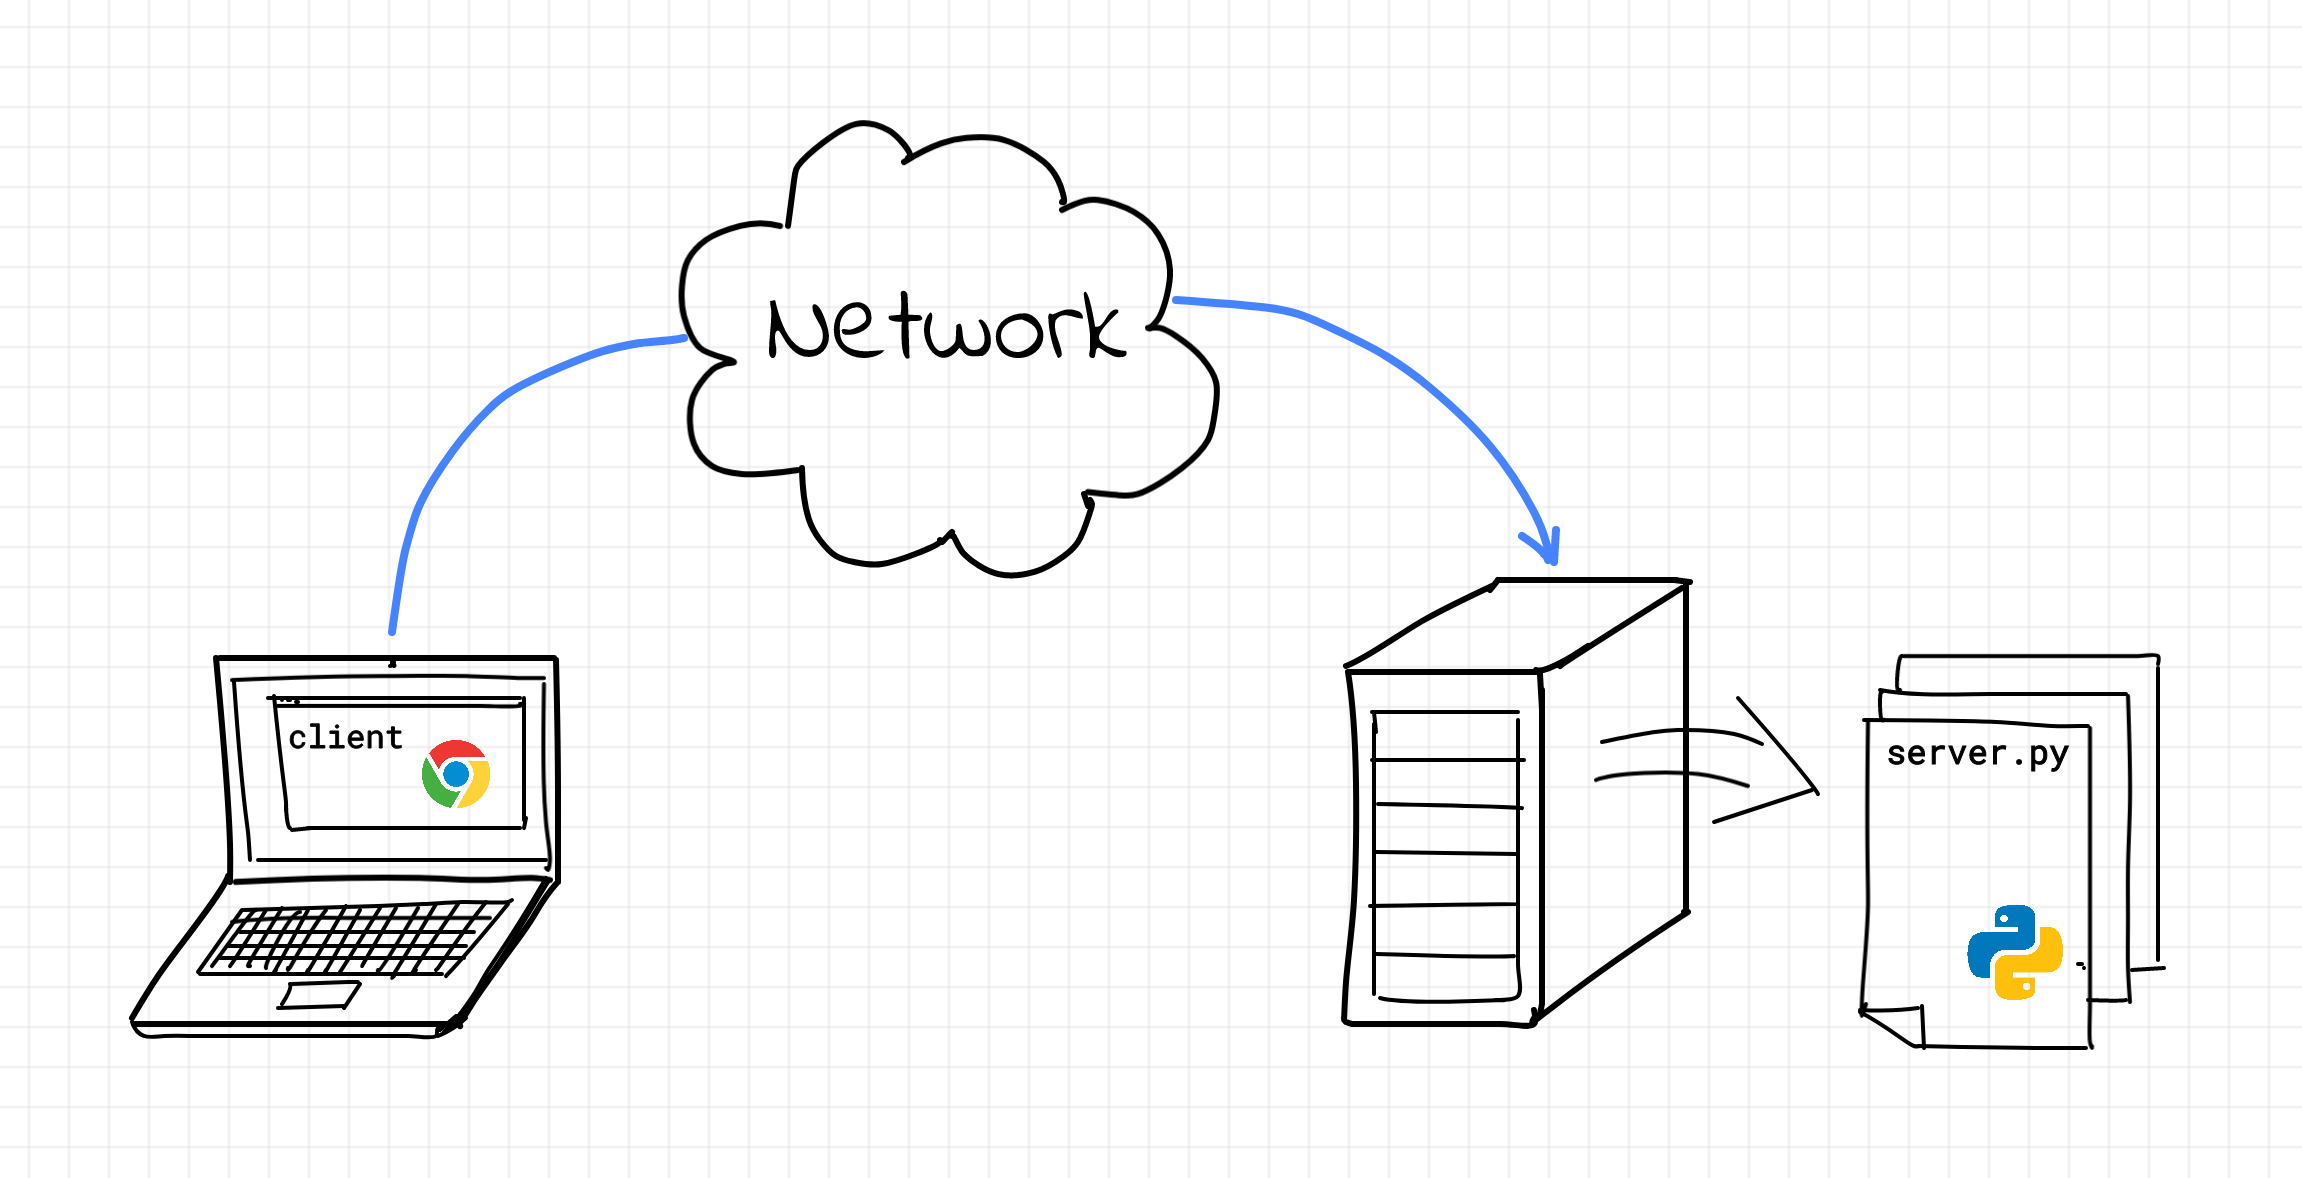
\includegraphics[width=10cm]{image/socket.png}
\end{center}
\caption{Mô hình Socket}
\end{figure}

Trong ngữ cảnh của lập trình mạng, một socket được coi là một đầu cuối của một kênh truyền thông giữa hai thiết bị. Một socket có thể hoạt động dựa trên nhiều giao thức truyền thông như TCP (Transmission Control Protocol) hoặc UDP (User Datagram Protocol).

\subsubsection{Lịch sử hình hành}
\hspace{5mm}
Socket là một khái niệm và công nghệ quan trọng trong lĩnh vực lập trình mạng. Được phát triển từ những năm 1970, socket đã trở thành một phần không thể thiếu trong việc xây dựng ứng dụng mạng hiệu quả.

Ban đầu, socket được phát triển bởi Ủy ban Nghiên cứu Mạng xã hội (ARPA) của Bộ Quốc phòng Hoa Kỳ (Hiện nay là Cục Nghiên cứu Dự án Tiên tiến - DARPA) như một phần của Dự án ARPANET, một mạng máy tính tiền thân của Internet. Socket được sử dụng để thiết lập kết nối và truyền thông giữa các máy tính trên mạng. Ban đầu, socket được viết bằng ngôn ngữ lập trình C.

Sau đó, socket được tiêu chuẩn hóa trong các tài liệu RFC (Request for Comments) của IETF (Internet Engineering Task Force), đặc biệt là RFC 793 "Transmission Control Protocol" và RFC 768 "User Datagram Protocol". Các RFC này định nghĩa giao thức TCP và UDP, và cung cấp cách sử dụng socket để truyền dữ liệu qua mạng bằng hai giao thức này

\subsubsection[short]{Một số ứng dụng của Socket}
\begin{itemize}
	\item \textbf{Truyền dữ liệu:} Socket được sử dụng để truyền dữ liệu giữa các máy tính trên mạng, bao gồm truyền tệp, tin nhắn, và dữ liệu khác.
	\item \textbf{Thiết lập kết nối:} Socket được sử dụng để thiết lập kết nối giữa các máy tính trên mạng, bao gồm kết nối TCP và UDP.
	\item \textbf{Xử lý giao thức:} Socket được sử dụng để xử lý các giao thức truyền thông như TCP và UDP, bao gồm việc gửi và nhận dữ liệu, xác định địa chỉ IP và cổng, và xử lý lỗi truyền thông.
	\item \textbf{Phát triển ứng dụng mạng:} Socket được sử dụng để phát triển ứng dụng mạng như trò chơi trực tuyến, ứng dụng trò chuyện, và ứng dụng chia sẻ tệp.
	\item \textbf{Kiểm tra mạng:} Socket được sử dụng để kiểm tra mạng bằng cách gửi và nhận dữ liệu giữa các máy tính trên mạng.
	\item \textbf{Bảo mật mạng:} Socket được sử dụng để bảo mật mạng bằng cách mã hóa dữ liệu trước khi truyền và giải mã dữ liệu sau khi nhận.
\end{itemize}

\subsubsection[short]{Ứng dụng Socket vào trong Pygame}
\hspace{5mm}
Ứng dụng của socket trong Pygame là tạo ra các trò chơi đa người chơi thông qua mạng. Bằng cách sử dụng socket, bạn có thể thiết lập kết nối mạng giữa các máy tính và truyền dữ liệu giữa chúng để tạo trải nghiệm chơi game đa người chơi. Dưới đây là một số ứng dụng của socket trong Pygame:
\begin{itemize}
	\item \textbf{Trò chơi đa người chơi:} Sử dụng socket để tạo ra các trò chơi đa người chơi trên mạng, bao gồm trò chơi đối kháng, trò chơi hợp tác, và trò chơi trực tuyến.
	\item \textbf{Trò chơi trực tuyến:} Sử dụng socket để tạo ra các trò chơi trực tuyến giữa các máy tính trên mạng, cho phép người chơi chơi cùng nhau từ xa.
	\item \textbf{Trò chơi địa phương:} Sử dụng socket để tạo ra các trò chơi địa phương giữa các máy tính trên cùng một mạng LAN, cho phép người chơi chơi cùng nhau trên cùng một mạng.
	\item \textbf{Trò chơi chia sẻ màn hình:} Sử dụng socket để chia sẻ màn hình giữa các máy tính trên mạng, cho phép người chơi xem và điều khiển trò chơi từ xa.

\end{itemize}





	% 	\begin{mdframed}[hidealllines=true,backgroundcolor=magenta!10]
	% 	\begin{lstlisting}
	% 	% ------------------------------- %
	% 	%     XOA MAN HINH VA CAC BIEN    %
	% 	% ------------------------------- %
	% 	clear
	% 	clc
		
	% 	% ------------------------------- %
	% 	%      NHAP DU LIEU BAI TOAN      %
	% 	% ------------------------------- %
	% 	n = ...;      % So nguoi dan
	% 	m = ...;      % So benh vien
	% 	% Ma tran D bieu dien thu tu uu tien cua benh vien doi voi benh nhan
	% 	% ung voi tung hang
	% 	D = [...];
	% 	% Ma tran B bieu dien thu tu uu tien cua benh nhan doi voi benh vien
	% 	% ung voi tung cot
	% 	B = [...];
	% 	% Ma tran c bieu dien suc chua cua tung benh vien
	% 	c = [...];
	% 	% Ma tran a bieu dien moi benh nhan chi duoc chon lua mot benh vien
	% 	a = ones(n,1);
		
	% 	% ------------------------------- %
	% 	% GIAI BAI TOAN BANG SOLVER MOSEK %
	% 	% ------------------------------- %
	% 	cvx_begin
	% 		cvx_solver mosek
	% 		% Bien x(i,j) chi nhan gia tri 0 hoac 1
	% 		% ung voi su ghep goi benh nhan r_i voi benh vien h_j
	% 		variable x(n,m) binary
	% 		% Toi da tong cac bien x(i,j)
	% 		% tuc la cang nhieu cap duoc ghep doi cang tot
	% 		maximize( 0 )
	% 		subject to
	% 			% Tong cac hang trong cung mot cot (so benh nhan duoc chon)
	% 			% nho hon hoac bang suc chua cua benh vien
	% 			sum(x,1) <= c;
	% 			% Tong cac cot trong cung mot cot (so benh vien duoc chon)
	% 			% nho hon hoac bang 1
	% 			sum(x,2) <= a;
	% 		% Bao dam khong co cac cap chan
	% 		for u = 1:n
	% 			for v = 1:m
	% 				%Tinh so hang dau tien trong ham dieu kien on dinh
	% 				t1 = 0;
	% 				for j = 1:m 
	% 					t1 = t1 + lt(D(u,j),D(u,v)) * x(u,j); 
	% 				end
	% 				%Tinh so hang thu hai trong ham dieu kien on dinh
	% 				t2 = 0;
	% 				for i = 1:n
	% 					t2 = t2 + lt(B(i,v),B(u,v)) * x(i,v) / c(v); 
	% 				end
	% 				%Xac lap ham dieu kien on dinh
	% 				t1 + t2 + x(u,v) >= 1;
	% 				%Ham dam bao cac cap (r_u,h_v) duoc xet nam trong A, neu
	% 				%cap do khong nam trong A thi x_uv = 0
	% 				if D(u,v) == m+n+1 || B(u,v) == m+n+1
	% 					(eq(D(u,v),m+n+1) + eq(B(u,v),m+n+1)) * x(u,v) == 0;
	% 				end
	% 			end
	% 		end
	% 	cvx_end
		
	% 	% ------------------------------- %
	% 	%  HIEN THI KET QUA RA MAN HINH   %
	% 	% ------------------------------- %
	% 	D
	% 	B
	% 	c
	% 	x       % Cac cap duoc ghep doi
	% \end{lstlisting}
	% \end{mdframed}
	% \subsection{Các công trình liên quan}
	% \textbf{ Giới thiệu vấn đề}
	% Công việc các bạn cần làm

\newpage
%%%%%%%%%%%%%%%%%%%%%%%%%%%%%%%%%
\section{Giới thiệu về Game Ping Pong}
\subsection{Lý do}
\subsection{Mục tiêu}
\subsection{Định hướng phát triển}


\newpage





%%%%%%%%%%%%%%%%%%%%%%%%%%%%%%%%%
\begin{thebibliography}{80}

\bibitem{CVX}
CVX Introduction
``\textbf{link: http://cvxr.com/cvx/doc/intro.html/}'',
\textit{What is CVX}, lần truy cập cuối: 15/04/2017.

\end{thebibliography}
\end{document}

